% $File: usage.tex
% $Date: Sat Jun 15 00:21:29 2013 +0800
% $Author: jiakai <jia.kai66@gmail.com>

\section{使用方法}
旋转部分有一个电源插口和两个开关,如图所示:
\begin{center}
	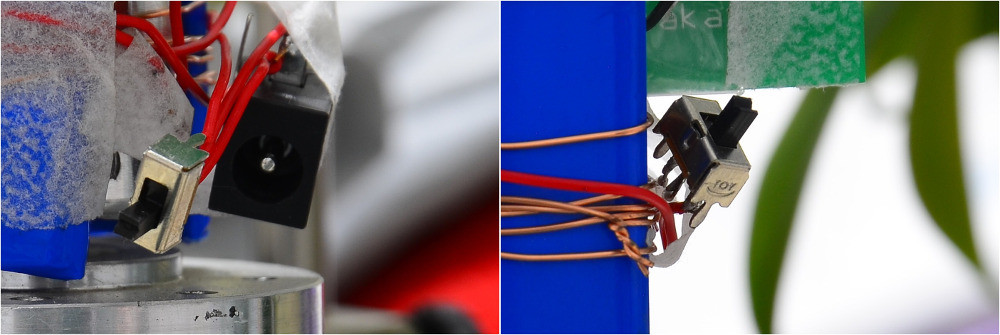
\includegraphics[width=0.8\textwidth]{../img/switch.png}
\end{center}
其中靠近电源插口的开关用于选择电源接法,
即在给电池充电和直接给电路板供电间切换;另一个开关用于选择电池是否给电路板供电。

使用时,先打开电池供电开关,电源指示灯点亮,再打开电动机;
由于电动机增加了限流电阻,需要用手拨动才能启动;启动后,
手持红外发射模块靠近旋转部分下方,系统检测到信号后,
即可计算转速并正确显示立体图形。最终效果如图所示,显示的是正四棱锥:
\begin{center}
	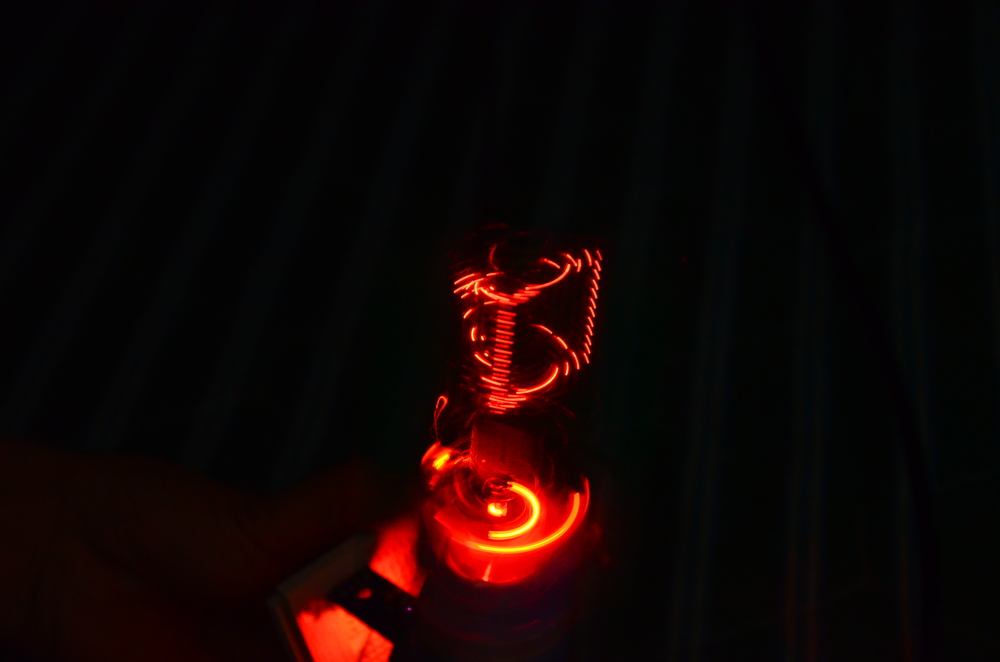
\includegraphics[width=0.5\textwidth]{../img/final.jpg}
\end{center}

% vim: filetype=tex foldmethod=marker foldmarker=f{{{,f}}}

